% JEPA -- joint-embedding predictive architecture.  Build: latexmk -pdf jepa.tex
\documentclass[border=8pt]{standalone}
\usepackage{amsmath}
% Shared TikZ palette + node styles for the ML-RT2 architecture diagrams.
% Colours match the ML-RT comparison-paper figures so the three papers look consistent:
%   pink   = data / vectors (inputs, outputs, latent representations)
%   blue   = learned networks / operators (MLPs, encoders, decoders, ...)
%   orange = special operations / physics (spectral transforms, RT residual, ...)
%   green  = loss / training terms
\usepackage{tikz}
\usetikzlibrary{arrows.meta,positioning,fit,backgrounds,calc}

\definecolor{dataFill}{HTML}{F2E6FF}\definecolor{dataDraw}{HTML}{6600CC}
\definecolor{netFill}{HTML}{B5E8E8}\definecolor{netDraw}{HTML}{086565}
\definecolor{opFill}{HTML}{FFE0C2}\definecolor{opDraw}{HTML}{AB4F03}
\definecolor{lossFill}{HTML}{C8F4C1}\definecolor{lossDraw}{HTML}{0C5600}

\tikzset{
  font=\small,
  box/.style  ={draw, rounded corners, align=center, inner sep=4pt, minimum height=9mm, line width=0.3mm},
  data/.style ={box, fill=dataFill, draw=dataDraw},
  net/.style  ={box, fill=netFill,  draw=netDraw},
  op/.style   ={box, fill=opFill,   draw=opDraw},
  loss/.style ={box, fill=lossFill, draw=lossDraw},
  sum/.style  ={draw=netDraw, circle, inner sep=1.3pt, fill=white, line width=0.3mm},
  arr/.style  ={-{Stealth[length=2.4mm]}, thick},
  darr/.style ={-{Stealth[length=2.4mm]}, thick, dashed},
  note/.style ={align=center, font=\scriptsize, text=black!65},
}

\begin{document}
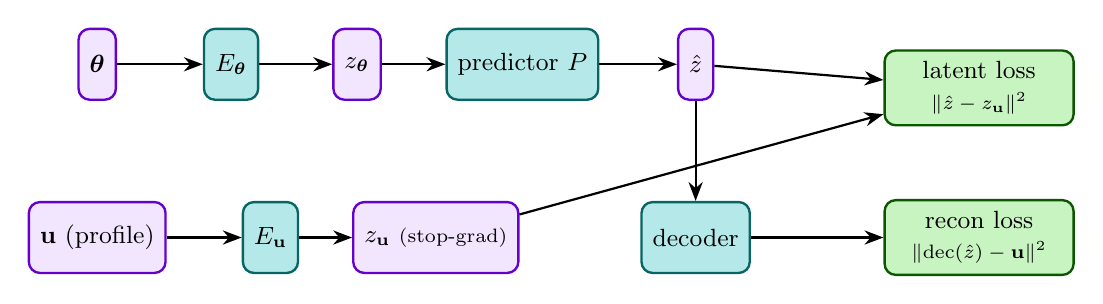
\begin{tikzpicture}
  % parameter path (top)
  \node[data] (th)  at (0,0)    {$\boldsymbol{\theta}$};
  \node[net]  (eth) at (1.7,0)  {$E_{\boldsymbol{\theta}}$};
  \node[data] (zth) at (3.3,0)  {$z_{\boldsymbol{\theta}}$};
  \node[net,  minimum width=16mm] (P) at (5.4,0) {predictor $P$};
  \node[data] (zh)  at (7.6,0)  {$\hat z$};
  \draw[arr] (th)--(eth); \draw[arr] (eth)--(zth); \draw[arr] (zth)--(P); \draw[arr] (P)--(zh);

  % profile path (bottom, provides the target embedding)
  \node[data, minimum width=15mm] (u)  at (0,-2.2)   {$\mathbf{u}$ (profile)};
  \node[net]  (eu) at (2.2,-2.2)  {$E_{\mathbf{u}}$};
  \node[data, minimum width=16mm] (zu) at (4.3,-2.2) {$z_{\mathbf{u}}$ {\scriptsize (stop-grad)}};
  \draw[arr] (u)--(eu); \draw[arr] (eu)--(zu);

  % decoder (lower) and the two loss boxes (far right, vertically aligned)
  \node[net]  (dec) at (7.6,-2.2)  {decoder};
  \node[loss, minimum width=24mm] (ll) at (11.2,-0.3) {latent loss\\{\scriptsize $\|\hat z - z_{\mathbf{u}}\|^2$}};
  \node[loss, minimum width=24mm] (rl) at (11.2,-2.2) {recon loss\\{\scriptsize $\|\mathrm{dec}(\hat z)-\mathbf{u}\|^2$}};

  \draw[arr] (zh) -- (ll);
  \draw[arr] (zh) -- (dec);
  \draw[arr] (dec) -- (rl);
  \draw[arr] (zu) -- (ll);
\end{tikzpicture}
\end{document}
